\section{Planificación y gestión del proyecto}
\setlength{\parskip}{0.5cm}

Los proyectos de software, evidentemente son proyectos ante todo, y por lo tanto van a tener características y procesos comunes a cualquier proyecto de ingeniería en general. Algunos de estos procesos que vamos a tratar en esta sección son: breve resumen de la necesidad de planificación, estimaciones acerca del tiempo que ha costado desarrollar la aplicación y en general invertido en el proyecto, estimaciones de costes y recursos necesarios para llevar a cabo dicho trabajo, estimación de los posibles riesgos que pueden surgir junto con sus posibles planes de contingencia y para finalizar hablaremos de la necesidad de la calidad del producto entregado cuando el proyecto tiene un marco temporal fijo y dinero limitado, que son las principales restricciones de los proyectos de este tipo. 

\textcolor{red}{quizá como una enumeración quedaría mejor}

\subsection{Necesidad de planificación}
Los proyectos software, como su nombre bien lo indica son proyectos, aunque a lo largo de la historia esta ultima parte se olvida a menudo. Desde que la informática comenzó en sus días, las empresas se embarcaban en grandes macro proyectos de cientos de miles de euros, pero la realidad es que muchos de ellos fracasaban y la principal de las razones era la falta de una adecuada planificación. Por lo menos con el tiempo, tanto las empresas como los profesionales y expertos en planificación han conseguido que esto no pase tanto, es decir, hay una tendencia alcista en lo que a éxitos en los proyectos de software se refiere, junto con un descenso significativo de los proyectos que al final no se acaban por unas u otras razones. 

La planificación es necesaria en todos los niveles, no hay ningún proyecto grande ni pequeño que se pueda empezar sin una planificación mínima. Incluso el proyecto más pequeño parte de una idea inicial que una persona tiene estructurada en la cabeza, lo cual es planificación. 

Cuando intentamos abordar proyectos de software que involucran a cientos de personas, recursos, cantidades grandes de dinero, se espera que ese proyecto salga adelante, pero la verdad es que ese proyecto solo saldrá adelante si se ha planificado y ejecutado de acuerdo a dicha planificación.

Uno de los principales problemas de la falta de planificación en los proyectos de software es la invisibilidad, por lo general planificar la construcción de un puente o el propio proyecto es mucho más vísale que la construcción de un artefacto de software. Otra de las principales características que dificultan la planificación es la complejidad. No es lo mismo intentar coordinar a 2 personas para que levanten un muro, que desarrollar una aplicación multiplataforma, están objetivamente demostrado que los proyectos de software son más complejos que los tradicionales por unidad de coste.

Estas y otras características son las que al final llevan a tener una planificación de proyectos pobre o deficiente, lo cual puede desembocar en la no realización del proyecto, o en la realización del mismo pero son sobrecostes o funcionalidad que no se han llegado a desarrollar. 



\subsection{Definición del alcance y objetivos}
\input{capitulos/planificacionGestion/alcance.tex}

\subsection{Tiempo de desarrollo}
La estimación en genera es una tarea complicada y difícil, yo en este documento voy a intentar reflejar mi mejor aproximación del tiempo que se va a invertir en este proyecto y además se contrastará con el tiempo que hasta ahora se está invirtiendo. 

Este proyecto cuenta con un marco temporal que en principio se considera fijo. Pongamos que la fecha límite que no se puede rebasar, para la cual todos los entregables y artefactos del proyectos han de estar terminados es el:

\textcolor{red}{hay que acabar esta parte de la estimación del tiempo, pero a dia de hoy me estreso solo vinedola ademas hay que establecerse hitos autopersonales}

\subsection{Recursos y costes}
\subsubsection{Recursos y tipos}

En lo que a estimación de recursos y costes se refiere, este proyecto es modesto, es decir que no va a disponer ni depender de caros y grandes recursos. Podemos tener varios tipos de recursos, al ser un proyecto pequeño, se van a dividir en 3 grandes categorías:
\begin{itemize}
\item \textbf{Personales}: a nivel de personal solo se involucran a 3 personas reales. Una es el director del TFG, a la cual no se le puede contar casi como recurso, ya que es mas la persona que desbloquea los principales problemas que nos podemos ir encontrando conforme vamos realizando el proyecto. Otra de las personas es el profesor asociado al cual va destinada la aplicación, esta persona si que es más importante porque hay otros recursos que han dependido de ella. Otro de los recursos personales es el propio autor del documento, el cual ha tenido que poner en práctica conocimientos de diseño de interfaces, software arquitectura, redacción... para lograr este documento. Luego haremos los cálculos de coste, de momento simplemente estamos planteando los recursos.

\item \textbf{Físicos}: a nivel de recursos físicos solo vamos a precisar de un ordenador para realizar el proyecto y la documentación del mismo, el ordenador no tiene que ser demasiado potente ya que solo tiene que cargar un IDE para desarrollar en aplicaciones Android. También podemos tener en cuenta los periféricos asociados y finalmente podemos añadir el móvil de pruebas en el que se van a realizar las principales pruebas físicas durante el desarrollo de la aplicación. 

\item \textbf{Datos}: voy a considerar como recursos los datos disponibles. Cuando empezó el trabajo la base de datos venía en forma de datos almacenados en un CD, pero en el futuro se ha visto que había por ejemplo falta de ese tipo de recursos.

\item \textbf{Otros}: podemos entrar a considerar recursos que para este proyecto no tiene casi sentido tener en cuenta. Dichos recursos pueden ser la electricidad gastada durante se desarrollaba el proyecto, o simplemente la estancia física donde se realizaba la acción. Repito que en este caso no tiene sentido tenerlos en cuenta pero si que me gustaría que quedase claro que en proyecto más grandes con muchas más personas, este tipo de recursos hay que contabilizarlos, controlarlos y tenerlos muy en cuenta (el precio de alquiler de una oficina puede disparar el precio de desarrollo por ejemplo).
\end{itemize}

\subsubsection{Estimación de los costes}

Intentar dar una estimación lo más adecuada posible de el coste de desarrollo total de este proyecto.
\begin{enumerate}
\item \textbf{Costes físicos}: estimar los costes de los recursos físicos anteriormente nombrados mediante la siguiente suma: 
$$ C_{fisico} = 550 + 20 + 15 + 150 = 735 EUR$$
El desglose sería el siguiente: 
\begin{enumerate}
\item \textbf{Ordenador}: por unos 550 EUR se pueden encontrar ordenadores con las prestaciones que nosotros buscamos. Mas o menos tienen que tener 8GB de RAM y con un procesador del tipo Intel Core i3 o i5 es suficiente. Con un almacenamiento de 500GB de disco HDD (no se precisan tantos) se puede desarrollar perfectamente este trabajo en condiciones buenas. 
\item \textbf{Ratón}: 20 EUR es el precio de mercado medio de un ratón inalámbrico para usarlo con el ordenador.
\item \textbf{Teclado}: 20 EUR es el precio de mercado medio de un teclado externo para usarlo con el ordenador.
\item \textbf{Móvil}: 150 EUR es el precio medio de un móvil con prestaciones normales, es decir entre 1GB y 2GB de RAM, almacenamiento ROM de entre ( y 16 GB y un procesador, junto con pantalla y cámaras de prestaciones medias. 
\end{enumerate}

\item \textbf{Costes personales}: para los costes personales primero tenemos que tener una buena estimación temporal, que en nuestro caso es: X días. Para ver cuanto cuesta pagar a una persona y que desarrollo dicho proyecto vamos a suponer que la hora a la que ese trabajador ha desarrollado el proyecto ha sido pagada a: 5 EUR, que dedicando una jornada laboral completa suponen unos beneficios de 40 EUR/dia y 1200 EUR/mes (no vamos a contabilizar los impuesto para facilitar las operaciones). Como nuestro trabajador va a dedicar unos X días, el coste de esa persona es aproximadamente: 
$$ C_{personal} = X dias \cdot 40 EUR/dia = XXXX EUR$$

\item \textbf{Costes totales}: los costes totales son los siguientes: 
$$ C_{total} = C_{fisico} + C_{personal} = 735 + XXXX EUR$$
\end{enumerate}

\textcolor{red}{acabar los calculo del coste, dependen del timpo}


\subsection{Tratamiento de los riesgos}
La gestión de riesgos es un tema complicado, que intentaré abordar según la mayor brevedad y facilidad posible. Aunque la planificación de un proyecto se basa en describir, planificar, asignar y revisar las tareas y recursos conocidos, existen muchos recursos desconocidos o difíciles de establecer que pueden incidir directamente en la consecución de los resultados en el tiempo previsto. Un riesgo implica dos factores claves:
\begin{itemize}
\item \textbf{Incertidumbre}: probabilidad de que dicho riesgo se manifieste con el paso del tiempo.
\item \textbf{Pérdida}: si el riesgo se convierte en una realidad, ocurrirán consecuencias o pérdidas no deseadas.
\end{itemize}

EL proceso de tratamiento de los riesgos tiene unas fases bien claras y definidas. Muchas empresas optan por la negación de los riesgos y la corrección de los mismos junto con los problemas ocasionados mientras estos van apareciendo. Este comportamiento no es mas que el reflejo de una pobre gestión y planificación ya que los riesgos son potenciales problemas que pueden surgir durante el desarrollo y si no se tienen en cuenta, pueden dar lugar a la no consecución de los objetivos del proyecto o incluso a la no finalización del mismo.

Vamos a dar unas pequeñas clasificaciones de posibles riesgos y luego presentaremos un análisis de riesgos inicial. Estamos por lo tanto en la \textbf{fase de análisis de riesgos}: 
\begin{itemize}
\item \textit{Directos}: depende enteramente de tu proyecto.
\item \textit{Indirectos}: tu proyecto no puede hacer nada, están fuera del alcance. 
\end{itemize}

Otro tipo de clasificación que podemos dar:
\begin{itemize}
\item \textit{De proyecto}: amenazan el plan del proyecto, aumentan el tiempo y el coste generalmente.
\item \textit{Técnicos}: potenciales riesgos de implementación, arquitectura, diseño ...
\item \textit{De negocio}: no entender bien los requisitos, no es de calidad, no es intuitivo. 
\end{itemize}

Hemos hablado de que estamos en la fase de análisis de riesgos, una vez que hemos clasificado los riesgos deberíamos de estimar la probabilidad de que estos sucedan y el impacto al proyecto en caos de que se manifiesten. Al terminar esta fase deberíamos de pensar en posibles soluciones y alternativas para los problemas que se pueden ocasionar si dicho riesgo se manifiesta en el futuro. En conclusión la lista de riesgos, junto con la probabilidad, el impacto y la posible solución la podemos revisar a continuación. Además dicha lista está ordenada por prioridad:

\begin{itemize}
\item \textbf{Pérdida repentina de datos del PC}: 10\% de que ocurra - 0.9 de impacto - Posible solución: usar tecnologías de almacenamiento en la nube junto con la replicación de los datos en varios soportes de almacenamiento. 
\item \textbf{Mala gestión del tiempo}: 40\% de que ocurra - 0.95 de impacto - Posible solución: posponer la presentación de dicho trabajo.
\item \textbf{Diseño poco intuitivo de la interfaz}: 10\% de que ocurra - 0.5 de impacto - Posible solución: organizar reuniones periódicas con el cliente para prevenir la aparición del riesgo.
\item \textbf{Mal diseño de la base de datos}: 10\% de que ocurra - 0.2 de impacto - Posible solución: para prevenir podemos diseñar la base de datos de las maneras aprendidas en la carrera, aunque a veces no sean los mejores diseño nos podemos aferrar a buenos diseños de manera objetiva si hemos cumplido ciertas reglas. 
\item \textbf{Falta de datos}: 50\% de que ocurra - 0.8 de impacto - Posible solución: hablar con los profesores encargados para buscar o generar dichos datos. (manifestado)
\item \textbf{Explotación pobre de la base de datos}: 10\% de que ocurra - 0.2 de impacto - Posible solución: organizar charlas con el cliente para que presente todas las ideas posibles. 
\item \textbf{Bloqueo a nivel técnico por el lenguaje de programación}: 5\% de que ocurra - 0.1 de impacto - Posible solución: usar otro lenguaje de programación o mejorar las habilidades en el que se está usando.
\item \textbf{Mala arquitectura de la aplicación}: 15\% de que ocurra - 0.5 de impacto - Posible solución: aplicar patrones bien definidos y estudiados por personalidades importantes dentro del mundo de la arquitectura de software. Esta comprobado de manera objetiva que son buenas soluciones a problemas que ya se han planteado con anterioridad. 
\item \textbf{Bajo rendimiento}: 5\% de que ocurra - 0.3 de impacto - Posible solución: optimizar las búsquedas en la base de datos, estructuras de datos de la aplicación ...
\item \textbf{Baja calidad del producto}: 20\% de que ocurra - 0.1 de impacto - Posible solución: someter a la aplicación a un sistema de integración continua donde se prueba una cierta y mínima calidad, tanto a nivel de código como de funcionamiento de software. 
\end{itemize}

\textcolor{red}{aun hay que ordenar los riesgos según una prioridad que tenemos que establecer, pensar mas riesgos}

\subsection{Control de configuraciones}
La gestión de la configuración en este proyecto no va a ser su punto fuerte. El objetivo de la gestión de la configuración es mantener la integridad de los artefactos que se obtienen en cada uno de los proyectos que integran el área garantizando que no se realizan cambios no controlados y que todos los participantes del proyecto disponen de la versión adecuada de los productos y artefactos que manejan. 

Así, entre los elementos de configuración software, se encuentran no únicamente ejecutables y código fuente, sino también los modelos de datos, modelos de procesos, especificaciones de requisitos, pruebas, etc. La gestión de configuración es una actividad continúa ya que se realiza durante todas las actividades asociadas al desarrollo de un sistema, y continúa registrando los cambios hasta que éste deja de utilizarse. Es una actividad de garantía de calidad que se aplica en todas las fases del proceso de ingeniería del software.

En nuestro caos no se va a usar un software específico de gestión de configuraciones. Además la gestión de configuraciones no es solo una base de datos donde se mantiene la información. Es un proceso continuo que avanza en paralelo al desarrollo del proyecto. Un ejemplo de una buena gestión de configuraciones habla de la necesidad de realizar auditorías, pero en un proyecto tan pequeño como el que vamos a desarrollar no tiene sentido.

En nuestro caso para mantener un mínimo control sobre las configuraciones y las versiones, no solo del código fuente y y de los ejecutables, sino también de los diagramas y de los documentos vamos a usar el mismo SCV que para el código fuente. Git. 

\subsection{Calidad de los productos entregados}
Hemos hablado de la posibilidad de una pobre calidad de los productos que entreguemos al final de nuestro proyecto. Hemos hablado que es un riesgo potencial y que en principio puede ser evitado o como mínimo prevenido. Durante el desarrollo de la aplicación vamos a asegurar el control de la calidad sometiendo el propio software a un proceso de desarrollo e integración continua. Como hemos mencionado de pasada en la parte de tecnologías, vamos a usar diferentes tecnologías para asegurarnos de que la calidad de nuestra aplicación es la máxima que le podemos ofrecer a nuestro cliente. 

La idea es que nosotros vamos a seguir un proceso de pruebas casi paralelo, aunque siempre un poco retrasado por definición en lo que a pruebas de sistema respecta, ya que probar la funcionalidad de algo, primero tenemos que desarrollarlo. 

Una vez estén implementadas las primeas interfaces de usuario, con sus principales interacciones es cuando se introducirán y diseñarán las principales pruebas de sistema. Además de estas pruebas se desarrollaran, aunque en menor medida pruebas funcionales para los módulos que se considere oportunos y que tengan un comportamiento esperado para una entrada dada. 

Todo este conjunto de pruebas se intentará que queden lo más automatizado posible. Como el objetivo principal es el desarrollo de la aplicación, no se le dará una importancia grande a esta parte, pero si que me gustaría introducir unas cuantas tecnologías de uso diario en el desarrollo ágil de productos software como puede ser Jenkins. Esta tecnología será la principal responsable de la automatización de toda nuestra suite de pruebas. Evidentemente no solo sirve para pruebas, sirve para automatizar procesos de software en general, otro ejemplo que podemos observar es el despliegue de un determinado servicio web en un entorno de desarrollo o producción cuando los cambios necesarios han sido realizados correctamente. 

Podemos ver en la \textbf{Figura \ref{fig:cicd}}, una aproximación del flujo al que se va a someter las diferentes partes de código que desarrollemos en nuestra aplicación.

\vspace{2cm}

\begin{figure}[H]
    \centering
    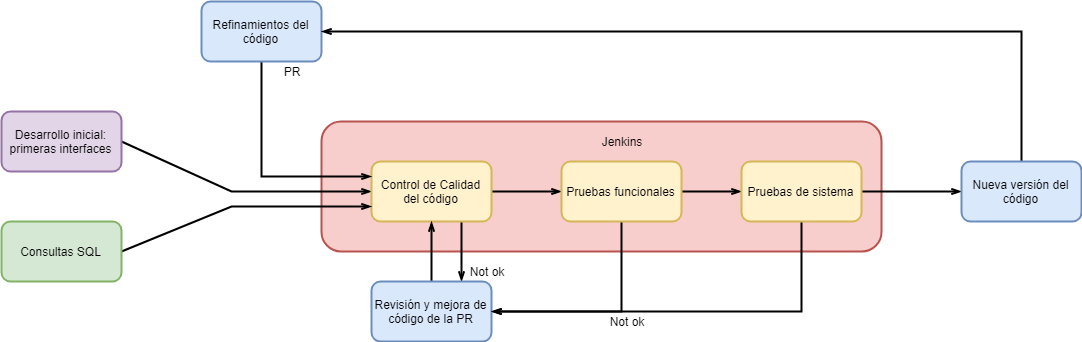
\includegraphics[scale=0.45]{imagenes/planificacionGestion/cicd.png}
    \caption{Flujo de Integración continua}
    \label{fig:cicd}
\end{figure}

\textcolor{red}{diseñar un pequeño diagrama del flujo que seguirán las pruebas y el código de la aplicación}